\chapter{Number theory}

\section{Modular arithmetic}
%	\kactlimport{ModularArithmetic.h}
	\kactlimport{ModInverse.h}
%	\kactlimport{ModPow.h}
	\kactlimport{ModLog.h}
	\kactlimport{ModSum.h}
	\kactlimport{ModMulLL.h}
	\kactlimport{ModSqrt.h}
	\kactlimport{Nimber.h}

\section{Primality}
	\kactlimport{FastEratosthenes.h}
	\kactlimport{MillerRabin.h}
	\kactlimport{Factor.h}

\section{Divisibility}
	\kactlimport{euclid.h}
	% \kactlimport{Euclid.java}
	\kactlimport{CRT.h}

	\subsection{Bézout's identity}
	For $a \neq $, $b \neq 0$, then $d=gcd(a,b)$ is the smallest positive integer for which there are integer solutions to
	$$ax+by=d$$
	If $(x,y)$ is one solution, then all solutions are given by
	$$\left(x+\frac{kb}{\gcd(a,b)}, y-\frac{ka}{\gcd(a,b)}\right), \quad k\in\mathbb{Z}$$

%\kactlimport{phiFunction.h}

\section{Fractions}
	\kactlimport{ContinuedFractions.h}
	\kactlimport{FracBinarySearch.h}

\section{Pythagorean Triples}
 The Pythagorean triples are uniquely generated by
 \[ a=k\cdot (m^{2}-n^{2}),\ \,b=k\cdot (2mn),\ \,c=k\cdot (m^{2}+n^{2}), \]
 with $m > n > 0$, $k > 0$, $m \bot n$, and either $m$ or $n$ even.

\section{Primes}
	$p=962592769$ is such that $2^{21} \mid p-1$, which may be useful. For hashing
	use 970592641 (31-bit number), 31443539979727 (45-bit), 3006703054056749
	(52-bit). There are 78498 primes less than 1\,000\,000.

	Primitive roots exist modulo any prime power $p^a$, except for $p = 2, a > 2$, and there are $\phi(\phi(p^a))$ many.
	For $p = 2, a > 2$, the group $\mathbb Z_{2^a}^\times$ is instead isomorphic to $\mathbb Z_2 \times \mathbb Z_{2^{a-2}}$.

\section{Estimates}
	$\sum_{d|n} d = O(n \log \log n)$.

	The number of divisors of $n$ is at most around 100 for $n < 5e4$, 500 for $n < 1e7$, 2000 for $n < 1e10$, 200\,000 for $n < 1e19$.
	Highly composite numbers: $8,96,840,9240,98280,997920,8648640,99459360$,\\
	$994593600,9777287520,97772875200,963761198400$,\\
	$9958865716800,97821761637600,978217616376000$,
	$9651747148243200,98930408269492800, 994651672331116800$

\section{Mobius Function}
\[
	\mu(n) = \begin{cases} 0 & n \textrm{ is not square free}\\ 1 & n \textrm{ has even number of prime factors}\\ -1 & n \textrm{ has odd number of prime factors}\\\end{cases}
\]
  Mobius Inversion:
  \[ g(n) = \sum_{d|n} f(d) \Leftrightarrow f(n) = \sum_{d|n} \mu(d)g(n/d) \]
  Other useful formulas/forms:

  $ \sum_{d | n} \mu(d) = [ n = 1] $ (very useful)

  $ g(n) = \sum_{n|d} f(d) \Leftrightarrow f(n) = \sum_{n|d} \mu(d/n)g(d)$

 $ g(n) = \sum_{1 \leq m \leq n} f(\left\lfloor\frac{n}{m}\right \rfloor ) \Leftrightarrow f(n) = \sum_{1\leq m\leq n} \mu(m)g(\left\lfloor\frac{n}{m}\right\rfloor)$

 \section{Irreducible polynomials over $\mathbb{F}_2$}

 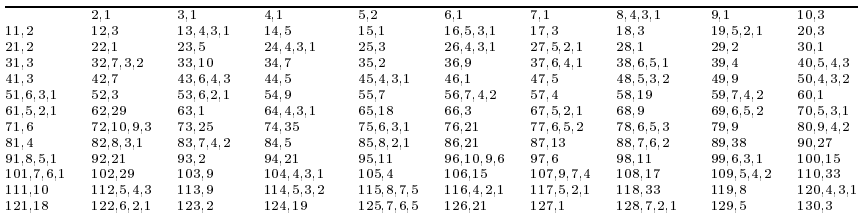
\includegraphics[width=9cm]{content/number-theory/table_pols.png}